\let\negmedspace\undefined
\let\negthickspace\undefined
\documentclass[journal]{IEEEtran}
\usepackage[a5paper, margin=10mm, onecolumn]{geometry}
%\usepackage{lmodern} % Ensure lmodern is loaded for pdflatex
\usepackage{tfrupee} % Include tfrupee package

\setlength{\headheight}{1cm} % Set the height of the header box
\setlength{\headsep}{0mm}     % Set the distance between the header box and the top of the text

\usepackage{gvv-book}
\usepackage{gvv}
\usepackage{cite}
\usepackage{amsmath,amssymb,amsfonts,amsthm}
\usepackage{algorithmic}
\usepackage{graphicx}
\usepackage{textcomp}
\usepackage{xcolor}
\usepackage{txfonts}
\usepackage{listings}
\usepackage{enumitem}
\usepackage{mathtools}
\usepackage{gensymb}
\usepackage{comment}
\usepackage[breaklinks=true]{hyperref}
\usepackage{tkz-euclide} 
\usepackage{listings}
% \usepackage{gvv}                                        
\def\inputGnumericTable{}                                 
\usepackage[latin1]{inputenc}                                
\usepackage{color}                                            
\usepackage{array}                                            
\usepackage{longtable}                                       
\usepackage{calc}                                             
\usepackage{multirow}                                         
\usepackage{hhline}                                           
\usepackage{ifthen}                                           
\usepackage{lscape}
\begin{document}

\bibliographystyle{IEEEtran}
\vspace{3cm}

\title{12.9.2.8}
\author{EE24BTECH11019 - Dwarak A}
% \maketitle
% \newpage
% \bigskip
{\let\newpage\relax\maketitle}

\renewcommand{\thefigure}{\theenumi}
\renewcommand{\thetable}{\theenumi}
\setlength{\intextsep}{10pt} % Space between text and floats


\numberwithin{equation}{enumi}
\numberwithin{figure}{enumi}
\renewcommand{\thetable}{\theenumi}

\textbf{Question:}\\
Consider the differential equation 
\begin{align}
    \brak{y\sin{y}+\cos{y}+x}y^\prime=y
    \label{eqn:ode}
\end{align}
    Verify that
\begin{align}
    x=y-\cos{y}
    \label{eqn:soln}
\end{align}
    is a solution for it

\solution

\medskip

\textbf{Theoretical Solution:}
\begin{align}
    y &= \frac{dy}{dx}\brak{y\sin{y}+\cos{y}+x} \\
    \frac{dx}{dy} - \frac{x}{y} &= \sin{y} + \frac{\cos{y}}{y}
\end{align}

Integrating factor,
\begin{align}
    \mu(y) &= e^{\int-\frac{1}{y}dy} \\
    \mu(y) &= \frac{1}{y}
\end{align}

Integration,
\begin{align}
    \frac{x}{y} &= \int\mu(y)\brak{\sin{y}+\frac{\cos{y}}{y^2}}dy \\
    \frac{x}{y} &= \int\frac{\sin{y}}{y}dy+\int\frac{\cos{y}}{y^2}dy \\
    \frac{x}{y} &= \int\frac{\sin{y}}{y}dy+\cos{y}\int\frac{1}{y^2}dy-\int\frac{\sin{y}}{y}dy \\
    \frac{x}{y} &= -\frac{\cos{y}}{y}+c \\
    x &= cy-\cos{y}
    \label{eqn:gen_soln}
\end{align}

Thus the equation \eqref{eqn:soln} is a solution to the differential equation \eqref{eqn:ode} when $c = 1$.

\medskip

\textbf{Algorithm (Forward Euler Method):}

Definition of derivative,
\begin{align}
    f^\prime(y) &\approx \lim_{h\to0}\frac{f(y+h)-f(y)}{h} \\
    f(y+h) &\approx f(y)+hf^\prime(y) \\
    \implies x_{n+1} &\approx x_{n} + h\frac{dx}{dy}\Big|_{x=x_{n}, y=y_{n}}
\end{align}

Difference equation,
\begin{align}
    x_{n+1} &\approx x_{n} + h\brak{\sin{y_{n} + \frac{\cos{y_{n}} + x_{n}}{y_{n}}}} \\
    y_{n+1} &= y_{n}+h
\end{align}

\begin{figure}[h]
    \centering
    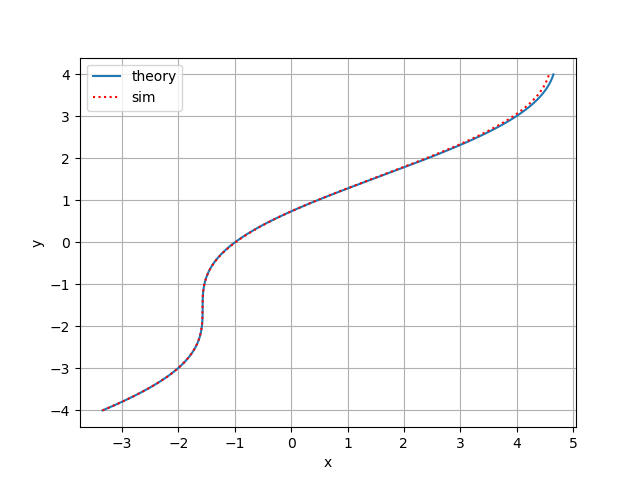
\includegraphics[width=\columnwidth]{figs/plot.png}
    \caption{Plot of the differential equation when $h=0.01$}
    \label{fig:Plot1}
    \end{figure}
\end{document}}
